\documentclass{article}

\usepackage{a4wide}
\usepackage {amsmath}
\usepackage{amssymb}
\usepackage {graphicx}
\usepackage[utf8]{inputenc} 
\usepackage[francais]{babel}
\usepackage{fancyhdr}
\usepackage{setspace}
\usepackage{fancyhdr}
\usepackage{lastpage}
\usepackage{extramarks}
\usepackage{chngpage}
\usepackage{soul}
\usepackage{algorithmicx} 
\usepackage{algpseudocode} 
\usepackage{multicol}
\usepackage[usenames,dvipsnames]{color}
\usepackage{graphicx,float,wrapfig}
\usepackage{ifthen}
\usepackage{listings}
\usepackage{courier}
\usepackage{esint}
\usepackage{bbm}
\usepackage{graphics}
\usepackage{graphicx}
\usepackage{subfig}
\usepackage{epsfig}
\usepackage{pgf,tikz}
\usetikzlibrary{arrows}
\usepackage{braket}
\usepackage{MnSymbol,wasysym}
\usepackage{marvosym}
\usepackage{dsfont}
 \usepackage{stmaryrd}
\usepackage{enumitem}
\usepackage{pst-node}
\usepackage{empheq}

% This is the color used for MATLAB comments below
\definecolor{MyDarkGreen}{rgb}{0.0,0.4,0.0}

% For faster processing, load Matlab syntax for listings
\lstloadlanguages{Matlab}%
\lstset{language=Matlab,                        % Use MATLAB
        frame=single,                           % Single frame around code
        basicstyle=\small\ttfamily,             % Use small true type font
        keywordstyle=[1]\color{Blue}\bf,        % MATLAB functions bold and blue
        keywordstyle=[2]\color{Purple},         % MATLAB function arguments purple
        keywordstyle=[3]\color{Blue}\underbar,  % User functions underlined and blue
        identifierstyle=,                       % Nothing special about identifiers
                                                % Comments small dark green courier
        commentstyle=\usefont{T1}{pcr}{m}{sl}\color{MyDarkGreen}\small,
        stringstyle=\color{Purple},             % Strings are purple
        showstringspaces=false,                 % Don't put marks in string spaces
        tabsize=5,                              % 5 spaces per tab
        %
        %%% Put standard MATLAB functions not included in the default
        %%% language here
        morekeywords={xlim,ylim,var,alpha,factorial,poissrnd,normpdf,normcdf},
        %
        %%% Put MATLAB function parameters here
        morekeywords=[2]{on, off, interp},
        %
        %%% Put user defined functions here
        morekeywords=[3]{FindESS, homework_example},
        %
        morecomment=[l][\color{Blue}]{...},     % Line continuation (...) like blue comment
        numbers=left,                           % Line numbers on left
        firstnumber=1,                          % Line numbers start with line 1
        numberstyle=\tiny\color{Blue},          % Line numbers are blue
        stepnumber=5                            % Line numbers go in steps of 5
        }

% Includes a MATLAB script.
% The first parameter is the label, which also is the name of the script
%   without the .m.
% The second parameter is the optional caption.
\newcommand{\matlabscript}[2]
  {\begin{itemize}\item[]\lstinputlisting[caption=#2,label=#1]{#1.m}\end{itemize}}
  
\newcommand{\cscript}[2]
  {\begin{itemize}\item[]\lstinputlisting[caption=#2,label=#1]{#1.c}\end{itemize}}

\newcommand{\gnuscript}[2]
  {\begin{itemize}\item[]\lstinputlisting[caption=#2,label=#1]{#1.gnu}\end{itemize}}
    
\begin{document}

 \title{Projet : méthode itérative des directions alternées (ADI)}

\author{Nathan Toussaint }
\date{\today}
%\date{\vspace{-10ex}}
 
 \maketitle
 
L'implémentation complète des différentes fonctions et des tests unitaires se trouvent dans les répertoires
de mon projet que j'ai nommés Q1 à Q6.

\section {Question 1}

La fonction {\tt Vec* buildVec(double val, int nx, int ny)} permet de construire un vecteur de réels double précision
de taille $n_x \times n_y$. Elle le crée de manière dynamique et retourne un pointeur $pt$ de type {\tt Vec*}.
On alloue d'abord $pt$ puis on procède le pointeur membre $pt->val$ pointant sur l'espace mémoire
où va être stocké les $n_x \times n_y$ valeurs réelles. On remarquera qu'à chaque appel de $malloc$,
on vérifie que l'allocation s'est bien déroulée sinon dans le cas contraire, on arrête le programme.
On remplit le tableau avec la même valeur $val$.

La fonction {\tt void destroyVec(Vec* pt)} désalloue l'espace mémoire, on libère d'abord l'espace pris
par le tableau de réels d'adresse mémoire $pt \rightarrow val$ puis on désalloue le pointeur $pt$.

La fonction {\tt Tridiag* buildM(double omega, int nl)} permet de construire de manière dynamique une matrice tridiagonale sous la forme de 3 vecteurs réels de taille $nl$. Elle retourne un pointeur $pt$ de type {\tt *Tridiag}.
On alloue d'abord $pt$ puis on procède à l'allocation des 3 tableaux $pt \rightarrow l$, $pt \rightarrow d$ et $pt \rightarrow u$.
Comme pour les vecteurs, on vérifie que l'allocation s'est bien passée.
On remplit ensuite le tableau grâce à une boucle pour construire $M(\omega)$. On annule les
composantes non pertinentes : la première composante de $pt \rightarrow l$ et la dernière de $pt \rightarrow u$.

La fonction {\tt void destroyM(Tridiag *pt)} désalloue l'espace mémoire, on libère d'abord l'espace pris
par les tableaux de réels d'adresses mémoires $pt \rightarrow l$, $pt \rightarrow d$ et $pt \rightarrow u$ puis on désalloue le pointeur $pt$.

\section{Question 2}

Dans une première partie, je décris l'algorithme de la décomposition $LU$ d'une matrice tri-diagonale $T$
stockée sous la forme de 3 vecteurs. Puis dans une seconde partie, je parle de son implémentation en C.

\subsection{Algorithme de la décomposition $LU$ d'une matrice tri-diagonale $T$}

On considère une matrice tridiagonale $T$ de dimension $N \times N$ :
\begin{equation}
T = \begin{pmatrix}
    d_0 & u_0 & 0 & \cdots & 0 \\
    l_1 & d_1 & u_1 & \ddots & \vdots \\
    0 & l_2 & d_2 & \ddots & 0 \\
    \vdots & \ddots & \ddots & \ddots & u_{n-2} \\
    0 & \cdots & 0 & l_{n-1} & d_{n-1}
\end{pmatrix}
\end{equation}
dont les termes diagonaux sont supposés non nuls.

On la stocke en mémoire sous la forme de 3 tableaux de même taille $N$ dont 
les indices commencent à 0 pour faciliter l'implémenation en C.
La diagonale de $T$ est stockée dans le tableau $d$, la première sous-diagonale dans $l$
et la première sur-diagonale dans $u$. On note que les composantes $0$ du vecteur $l$ et la composante $n-1$ du vecteur $u$ ne sont pas pertinentes.

La décomposition LU consiste à écrire la matrice tridiagonale $T$ sous la forme d'un produit $LU$ où
\begin{equation}
L = \begin{pmatrix}
    1 & 0 & 0 & \cdots & 0 \\
    \beta_1 & 1 & 0 & \ddots & \vdots \\
    0 & \beta_2 & 1 & \ddots & 0 \\
    \vdots & \ddots & \ddots & \ddots & 0 \\
    0 & \cdots & 0 & \beta_{n-1} & 1
\end{pmatrix}
\text{\quad et \quad}
U = \begin{pmatrix}
    \alpha_0 & u_0 & 0 & \cdots & 0 \\
    0  & \alpha_1 & u_1 & \ddots & \vdots \\
    0 & 0 &  \ddots & \ddots & 0 \\
    \vdots & \ddots & 0  &\alpha_{n-2} & u_{n-2} \\
    0 & \cdots & 0 & 0 & \alpha_{n-1}
\end{pmatrix}
\end{equation}

Comme la première sur-diagonale supérieure de $U$ s'identifie à celle de la matrice $T$,
 l'algorithme de décomposition LU se simplifie grandement.
 Une première version s'écrit:\\

\begin{algorithmic}[1]
\Function{LU}{$T$}
\State $\alpha_0 \gets d_0$
\For {$k = 1 ..  (n-1)$} 
	\State $\beta_k \gets l_k/\alpha_{k-1}$
	\State $\alpha_k \gets d_k -u_{k-1} \; \beta_k$
\EndFor                 
\EndFunction
\end{algorithmic}

Grâce à la structure tri-diagonale de $T$, il n'est pas nécessaire d'allouer une matrice supplémentaire
pour stocker la décomposition $LU$. Elle peut remplacer progressivement la matrice $T$ ligne par ligne.
L'algorithme optimisé en place mémoire s'écrit finalement : \\

\begin{algorithmic}[1]
\Function{LU}{$T$} \Comment {à la place de la matrice tridiagonale $T$}
\For {$k = 1 ..  (n-1)$} 
	\State $l_k \gets l_k/d_{k-1}$
	\State $d_k \gets d_k -u_{k-1} \; l_k$
\EndFor                 
\EndFunction
\end{algorithmic}

On note que la complexité de la décomposition $LU$ pour une matrice tri-diagonale de rang $N$ est $\vartheta(N)$.
Elle est donc peu couteuse par rapport à celle en $\vartheta(N^3)$ pour une matrice pleine de rang $N$.

\subsection{Implémentation}

\cscript{invM}{Construction de la décomposition $LU$}

\section{Question 3}

On suppose que la matrice $T$ a été décomposée en un produit $LU$ où $L$ est une matrice bi-diagonale inférieure
avec des $1$ sur la diagonale et $U$ est une matrice bi-diagonale supérieure dont les termes diagonaux sont non nuls.

Résoudre $LU x=b$ s'effectue en deux étapes : i) résolution de $L y=b$ par la méthode de descente pui ii) résolution
de $U x=y$ par la méthode de montée.

\subsection{Résolution de $ L y=b$ par la méthode de descente}

Soit le système d'équations linéaires où la matrice associée est bi-diagonale inférieure:

\begin{equation}
\begin{pmatrix}
    1 & 0 & 0 & \cdots & 0 \\
    l_1 & 1 & 0 & \ddots & \vdots \\
    0 & l_2 & 1 & \ddots & 0 \\
    \vdots & \ddots & \ddots & \ddots & 0 \\
    0 & \cdots & 0 & l_{n-1} & 1
\end{pmatrix}
\begin{pmatrix}
   y_0 \\
   y_1 \\
    \vdots\\
    \vdots \\
    y_{n-1}
\end{pmatrix}
=
\begin{pmatrix}
   b_0 \\
   b_1 \\
    \vdots\\
    \vdots \\
    b_{n-1}
\end{pmatrix}
\end{equation}

La méthode de résolution est celle de la descente. De nouveau, dans le cas de matrice bi-diagonale,
l'algorithme se simplifie et s'écrit:

\begin{algorithmic}[1]
\Function{DESCENTE}{$LU, b$}
\State $y_0 \gets b_0$
\For {$k = 1 ..  (n-1)$} \State $y_k \gets b_k-l_k \; y_{k-1}$
\EndFor                 
\EndFunction
\end{algorithmic}

La complexité de cet algorithme est $\vartheta(N)$.

\subsection{Résolution de $ U x= y$ par la méthode de montée}

Soit le système d'équations linéaires où la matrice associée est bi-diagonale supérieure:
\begin{equation}
U = \begin{pmatrix}
    d_0 & u_0 & 0 & \cdots & 0 \\
    0  & d_1 & u_1 & \ddots & \vdots \\
    0 & 0 &  \ddots & \ddots & 0 \\
    \vdots & \ddots & 0  &d_{n-2} & u_{n-2} \\
    0 & \cdots & 0 & 0 & d_{n-1}
\end{pmatrix}
\begin{pmatrix}
   x_0 \\
   x_1 \\
    \vdots\\
    x_{n-2} \\
    x_{n-1}
\end{pmatrix}
=
\begin{pmatrix}
   y_0 \\
   y_1 \\
    \vdots\\
    y_{n-2} \\
    y_{n-1}
\end{pmatrix}
\end{equation}

L'algorithme de la méthode de la montée s'écrit dans notre cas :
\begin{algorithmic}[1]
\Function{MONTEE}{$LU, y$}
\State $x_{n-1} \gets y_{n-1}/d_{n-1}$
\For {$i = (n-2) .. 1$} \State $x_k \gets (y_k-u_k \; x_{k+1}) / d_k$
\EndFor                 
\EndFunction
\end{algorithmic}

La complexité de cet algorithme est $\vartheta(N)$.

%\subsection{Complexité}
%
%La complexité de résolution d'un système tri-diagonale en utilisant la méthode de décomposition $LU$ et les
%méthodes de descente et de montée est $\vartheta(N)$ et peu couteuse par rapport à la méthode
%de résolution de Gauss qui a une complexité $\vartheta(N^3)$  pour une matrice dense de rang $N$.
 
\subsection{implémentation de la méthode de résolution}
  
L'implémentation se trouve dans le répertoire $Q3/0\_solveLU$. On a mis en oeuvre le cas test suivant
(voir main.c):
\begin{enumerate}
\item Création dynamique d'une matrice $M(\omega=1)$ de rang $nl=6$.
\item Création dynamique de deux vecteurs $RHS$ rempli de $1$ et $X$ rempli de $0$, de dimension $nl=6$ .
\item Résolution de $M X =RHS$. 
\item Comme la décomposition $LU$ remplace les valeurs de $M$. Il est nécessaire de le détruire
et de le reconstruire.
\item Vérification que $||RHS-M X||_\infty \rightarrow 0$.
\end{enumerate}

\subsection {Méthode de résolution ADI}

 On cherche à résoudre en 2D, l'équation de Poisson  : $-\Delta u(x,y)=f(x,y)$ sur un domaine carré $\Omega=]0, 1[^2$.
 Elle est discrétisée en différences finies sur une grille est de taille $n_x \times n_y$. 
 On impose des conditions de Dirichlet sur le contour $\partial \Omega$ épousant le contour de la grille : $u(x,y)=u^d(x,y)$
 ({\it notation différente du sujet pour réduire les ambiguités de notations avec les indices}).
 
 \subsection{Discrétisation du domaine carré}
 
 On repère chaque noeud de la grille par ses coordonnées entières $(i,j)$ comme dans l'exemple ci-dessous d'une grille
 $5 \times 4$ :
 
 \begin{table}[h]
\begin{center}
\begin{tabular}{ c c c }
\begin{tikzpicture}[scale=1.5]
  \draw (0,0) grid (4,3);
  \foreach \x in {0. ,1. ,...,4.}
    \foreach \y in {0.,1.,...,3.}
      \node at (\x+0.3,\y+0.15) {(\pgfmathparse{int(\x)}\pgfmathresult, \pgfmathparse{int(\y)}\pgfmathresult)};
      
        % Repère cartésien
  \draw[->] (0,0) -- (4.5,0) node[right] {$i$};
  \draw[->] (0, 0) -- (0,3.5) node[above] {$j$};
  
\end{tikzpicture}
\end{tabular}
    \caption{coordonnées entières des noeuds de la grille $5 \times 4$}
    \label{tab:CoordGrille}  
 \end{center}
\end{table}

 Dans l'approximation des différences finies, on définit :
 \begin{equation}
  \left. \hat{ L}_x u \right|_{(i,j)}=\left. -\partial_x^2 u \right|_{(i,j)} = \frac{-u(i-1,j)+2 u(i,j)-u(i+1,j)}{h_x^2}
+ \vartheta(h_x^2)
\end{equation}

 et 
  \begin{equation}
  \left. \hat{L}_y u  \right|_{(i,j)}=\left. -\partial_y^2 u  \right|_{(i,j)}=  \frac{-u(i,j-1)+2 u(i,j)-u(i,j+1)}{h_y^2} + \vartheta(h_y^2)
  \end{equation}
 
 où $h_x=\frac{1}{n_x-1}$ et $h_y=\frac{1}{n_y-1}$ sont les pas de la grille.
 
 Dans la suite, on introduit les notations $m_x =h_x^{-1} = n_x-1$ et $m_y=h_y^{-1}=n_y -1$.

Notons que la fonction $f(x,y)$ est évaluée aux noeuds intérieurs $(i,j)$ de la grille. 

%\begin{table}[h]
%\begin{center}
%\begin{tabular}{ c c c }
%\begin{tikzpicture}
%  \draw (0,0) grid (4,3);
%  \foreach \x in {0. ,1. ,...,4.}
%    \foreach \y in {0.,1.,...,3.}
%      \node at (\x+0.15,\y+0.15) {\pgfmathparse{int(\x+5*(\y))}\pgfmathresult};
%\end{tikzpicture}
%(a)
%&
%\quad \quad
%&
%\begin{tikzpicture}
%  \draw (0,0) grid (4,3);
%  \foreach \x in {0. ,1. ,...,4.}
%    \foreach \y in {0.,1.,...,3.}
%      \node at (\x+0.15,\y+0.15) {\pgfmathparse{int(5*\x+(\y))}\pgfmathresult};
%\end{tikzpicture}
%(b)
%\end{tabular}
%    \caption{Numérotations de la grille $5 \times 4$ en utilisant $n(i,j)=i+j\; n_x$  (a) puis $\bar {n}(i,j)=j+i\; n_y$ (b)}
%    \label{tab:NumGrille}   
% \end{center}
%\end{table}

%\noindent
% L'avantage de la numérotation (a) permet d'écrire de manière la plus compacte :
%   \begin{equation}
% \left. \hat{ L}_x u \right|_{n} = -m_x^2 \; u_{n-1} +2 m_x^2 \; u_n -m_x^2 \; u_{n+1} \text{\quad avec \quad} n(i,j)=i+j\; n_x
%   \end{equation}
%pour tout point intérieur $(i,j)$ de $\Omega$
%tandis que la numérotation (b) étant mieux adaptée pour $L_y$ :
%    \begin{equation}
% \left. \hat{L}_y u \right|_{\bar{n}} = -m_y^2 \; u_{\bar{n}-1} +2 m_y^2 \; u_{\bar{n}} -m_y^2 \; u_{\bar{n}+1}
% \text{\quad avec \quad} \bar{n}(i,j)=j+i\; n_y
%   \end{equation}
%en notant $m_x =h_x^{-1} = n_x-1$ et $m_y=h_y^{-1}=n_y -1$.
 
 \subsection{Les pas fractionnaires de la méthode}
    
La méthode de résolution ADI est une méthode itérative composée de deux pas fractionnaires.
Elle se caractérise par une approche qui alterne entre les directions x et y, en résolvant chaque sous-problème de manière implicite :

 \begin{eqnarray}\left\{ 
\begin{array}{lcl}
  (L_x+\omega_k I) u^* &=& -(L_y-\omega_k I) u^k +b \\
  \\
 (L_y+\omega_k I) u^{k+1} &=& -(L_x-\omega_k I) u^* +b \end{array} \right. 
  \label{ADI}
  \end{eqnarray}
  
Cette alternance permet de transformer la résolution de l'équation bidimensionnelle en deux problèmes unidimensionnels plus simples, qui peuvent être résolus efficacement.
En pratique, la résolution s'arrête lorsque  $||(L_x+L_y) \; u^k -b||_\infty < \epsilon$ avec $\epsilon \approx 10^{-6}$
par exemple, voire plus petit.

 \subsection{Application à la grille $5 \times 4$}
 
On propose de détailler la méthode ADI dans le cas d'une grille de taille $n_x \times n_y = 5 \times 4$. Le premier pas fractionnaire de la méthode ADI consiste à résoudre, pour chacune des lignes $j \in ]0, n_y-1[=\{1, 2\}$. Pour $i \in [1, 3]$, il s'écrit :
\begin{equation}
-m_x^2 u^*_{i-1, j} +(2m_x^2+\omega) u^*_{i, j} -m_x^2 u^*_{i+1, j} =
m_y^2 \; u_{1, j-1}^k - (2m_y^2-\omega)\; u_{1, j}^k +m_y^2 \; u_{1, j+1}^k
+b_{i,j}
\end{equation}
Viennent ensuite s'ajouter les conditions de dirichlet en $i=0$ et $i=n_x-1$.
\noindent
De manière matricielle, le système d'équations à résoudre s'écrit:
\begin{equation}
\begin{pmatrix}
    1 & 0 & 0 & 0 & 0 \\
    -m_x^2 & 2m_x^2+\omega & -m_x^2  & 0 & 0 \\
    0 &  -m_x^2 & 2m_x^2+\omega & -m_x^2  & 0 \\
    0 & 0 &  -m_x^2 & 2m_x^2+\omega & -m_x^2  & \\
    0 & 0 & 0 & 0 & 1
\end{pmatrix}
\begin{pmatrix}
   u^*_{0, j}\\
   u^*_{1, j}\\
   u^*_{2, j}\\
   u^*_{3, j}\\
   u^*_{4, j} \\
\end{pmatrix} = \\
\begin{pmatrix}
   0\\
   m_y^2 \; u_{1, j-1}^k - (2m_y^2-\omega)\; u_{1, j}^k +m_y^2 \; u_{1, j+1}^k \\
   m_y^2 \; u_{2, j-1}^k - (2m_y^2-\omega)\; u_{2, j}^k +m_y^2 \; u_{2, j+1}^k \\
   m_y^2 \; u_{3, j-1}^k - (2m_y^2-\omega)\; u_{3, j}^k +m_y^2 \; u_{3, j+1}^k \\
   0 \\
\end{pmatrix}
+
\begin{pmatrix}
   u^d_{0, j}\\
   b_{1, j}\\
   b_{2, j}\\
   b_{3, j}\\
   u^d_{4, j} \\
\end{pmatrix}
\end{equation}
où $u^d_{i,j}$ est la valeur de dirichlet au noeud de coordonnées $(i,j)$.
Cette première étape revient à résoudre $n_y-2$ petits systèmes linéaires dont la matrice est tri-diagonale de rang $n_x$.

De manière similaire, le second pas fractionnaire revient à résoudre, pour chacune des colonnes $i \in ]0, n_x-1[=\{1, 2, 3\}$ :
\begin{equation}
\begin{pmatrix}
    1 & 0 & 0 & 0  \\
    -m_y^2 & 2m_y^2+\omega & -m_y^2  & 0  \\
    0 &  -m_y^2 & 2m_y^2+\omega & -m_y^2  \\
    0 & 0 & 0 &  1
\end{pmatrix}
\begin{pmatrix}
   u^{k+1}_{i, 0}\\
   u^{k+1}_{i, 1}\\
   u^{k+1}_{i, 2}\\
   u^{k+1}_{i, 3}\\
\end{pmatrix} = \\
\begin{pmatrix}
   0\\
   m_x^2 \; u_{i-1, 1}^* - (2m_x^2-\omega)\; u_{i, 1}^* +m_x^2 \; u_{i+1, 1}^* \\
   m_y^2 \; u_{i-1, 2}^* - (2m_x^2-\omega)\; u_{i, 2}^* +m_y^2 \; u_{i+1, 2}^* \\
   0 \\
\end{pmatrix}
+
\begin{pmatrix}
   u^d_{i, 0}\\
   b_{i, 1}\\
   b_{i, 2}\\
   u^d_{i, 4} \\
\end{pmatrix}
\end{equation}

De même, cette seconde étape revient à résoudre $n_x-2$ petits systèmes linéaires dont la matrice est tri-diagonale de rang $n_y$.

Dans l'implémentation, on ne traitera que le cas où les valeurs de $u$ au bord sont strictement nulles.

\begin{table}[h]
\begin{center}
\begin{tabular}{ c c c }
\begin{tikzpicture}[scale=1.5]
  % Grille avec des valeurs entières
  \draw (0,0) grid (3,3);
  \foreach \x in {0,1,...,3}
    \foreach \y in {0,1,...,3}
      \node at (\x+0.15,\y+0.15) {\pgfmathtruncatemacro{\value}{int(\x)+4*int(\y)}\value};

  % Repère cartésien
 %\draw[->] (0,0) -- (4.5,0) node[right] {$i$};
 %\draw[->] (0, 0) -- (0,3.5) node[above] {$j$};
\end{tikzpicture}

\end{tabular}
    \caption{Numérotation unique des noeuds de la grille $4 \times 4$}
    \label{tab:NumGrille}  
 \end{center}
\end{table}

\subsection{Stockage des valeurs aux noeuds sous la forme d'un vecteur}



Du point de vue de l'implémentation, on stockera les approximations de la solution dans un tableau unidimensionnel 
de taille $n_x \times n_y$ en utilisant la relation $n(i,j)=i+j\; n_x$ qui numérote de manière unique chaque noeud $(i,j)$. 

\subsection{Implémentation de computeRHS}

L'implémentation se trouve dans le répertoire {\tt Q3/1\_computeRHS\_solve}. 
Je mets en oeuvre la présentation de la méthode ADI faite dans une précédente section.

La fonction {\tt void computeRHSX(int j, double omega, Vec *ptX, Vec *ptB, Vec *ptRHS)} construit
le second membre pour la ligne j, argument supplémentaire que j'ai ajouté par rapport à l'énoncé,
pour le premier pas fractionnaire.

La fonction {\tt void computeRHSY(int i, double omega, Vec *ptX, Vec *ptB, Vec *ptRHS)} fait de même
pour la colonne i.

La programme principal {\tt main.c} montre l'enchainement  des 2 pas fractionnaires.
Pour chacune des lignes (resp. chacune des colonnes), on a 
\begin{enumerate}
\item Contruction de la matrice $M$ et du second membre.
\item Résolution du système tridiagonale associé.
\item Mise à jour de la solution intermédiaire.
\item Libération de l'espace mémoire.
\end{enumerate}

\cscript{computeRHS\_main}{Appel des fonctions computeRHSX et computeRHSY }

 \section{Convergence}
    
On note $\bar u$ la solution de $(L_x+L_y) \bar u =b$. On définit les erreurs $\epsilon^k = u^k-\bar u$ et
$\epsilon^{*}= u^{*}-\bar u$.  En soustrayant $(L_x+L_y) \bar u =b$ des équations \eqref{ADI},
on obtient :
 \begin{eqnarray}\left\{ 
\begin{array}{lcl}
  (L_x+\omega_k I) \epsilon^{*} &=& -(L_y-\omega_k I) \epsilon^k \\
  \\
 (L_y+\omega_k I) \epsilon^{k+1} &=& -(L_x-\omega_k I) \epsilon^{*}  \end{array}  \right. 
  \label{err}
  \end{eqnarray}
 
Après élimination de $e^{*}$, on obtient :
\begin{equation}
 \epsilon^{k+1} = (L_y+\omega I)^{-1}  (L_x-\omega I)  (L_x+\omega I)^{-1} (L_y-\omega I) \; \epsilon^k = T(\omega) \epsilon^k
 \label{err}
\end{equation}
où
\begin{equation}
T(\omega) = (L_y+\omega I)^{-1} (L_x-\omega I)   (L_x+\omega I)^{-1} (L_y-\omega I)
 \label{Tk}
\end{equation}

A titre d'exemple,  prenons $n_x=n_y=4$, les matrices $L_x$ et $L_y$
en tenant compte des conditions de dirichlet sur les bords sont de la forme:

\begin{center}
\resizebox{\textwidth}{!}{%
   $L_x=$
   \begin{tabular}{| c | c | c | c | c | c | c | c | c | c | c | c | c | c | c | c | c | }
     \hline
     &0. & 1. & 2. & 3. & 4. & 5. & 6. & 7. & 8. & 9. & 10 & 11 & 12 & 13 & 14 & 15 \\ \hline
     0 & 1  &   &   &   &   &   &   &   &  &  &  &  &  &  &  &\\ \hline
     1 &  & 1  &   &   &   &   &   &   &  &  &  &  &  &  &  &\\ \hline
     2 &  &   &  1 &   &   &   &   &   &  &  &  &  &  &  &  &\\ \hline
     3 &  &   &   &  1 &   &   &   &   &  &  &  &  &  &  &  &\\ \hline
     4 &  &   &   &   &  1 &   &   &   &  &  &  &  &  &  &  &\\ \hline
     5 &  &   &   &   &  $-m_x^2$ &   $2 m_x^2$&  $-m_x^2$ &   &  &  & & &  &  &  &\\ \hline
     6 &   &  &   &   &   &  $-m_x^2$ &   $2 m_x^2$&  $-m_x^2$ &   &  &  & & &  &  & \\ \hline
     7 &  &   &   &   &   &   &   &  1  &  &  &  &  &  &  &  &\\ \hline
     8 &  &   &   &   &   &   &   &   & 1 &  &  &  &  &  &  &\\ \hline     
     9 & &  & & &  &   &   &   &  $-m_x^2$ &   $2 m_x^2$&  $-m_x^2$ &   &  &  &  &\\ \hline
   10 &  & &  & & &  &   &   &   &  $-m_x^2$ &   $2 m_x^2$&  $-m_x^2$ &   &  &   &\\ \hline
   11 &  &   &   &   &   &   &   &   &  &  &  & 1  &  &  &  &\\ \hline    
   12 &  &   &   &   &   &   &   &   &  &  &  &  & 1  &  &  &\\ \hline    
   13 &  &   &   &   &   &   &   &   &  &  &  &  &  & 1  &  &\\ \hline    
   14 &  &   &   &   &   &   &   &   &  &  &  &  &  &  &  1 &\\ \hline    
   15 &  &   &   &   &   &   &   &   &  &  &  &  &  &  &  & 1\\ \hline    
   \end{tabular}  
   }
 \end{center}

\begin{center}
\resizebox{\textwidth}{!}{%
   $L_y=$
   \begin{tabular}{| c | c | c | c | c | c | c | c | c | c | c | c | c | c | c | c | c | }
     \hline
     &0. & 1. & 2. & 3. & 4. & 5. & 6. & 7. & 8. & 9. & 10 & 11 & 12 & 13 & 14 & 15 \\ \hline
     0 & 1  &   &   &   &   &   &   &   &  &  &  &  &  &  &  &\\ \hline
     1 &  & 1  &   &   &   &   &   &   &  &  &  &  &  &  &  &\\ \hline
     2 &  &   &  1 &   &   &   &   &   &  &  &  &  &  &  &  &\\ \hline
     3 &  &   &   &  1 &   &   &   &   &  &  &  &  &  &  &  &\\ \hline
     4 &  &   &   &   &  1 &   &   &   &  &  &  &  &  &  &  &\\ \hline
     5 &  & $-m_y^2$   &   &   &   &   $2 m_y ^2 $&   &   &  &   $-m_y^2$ & & &  &  &  &\\ \hline
     6 &   &  & $-m_y^2$   &   &   &   &   $2 m_y ^2 $&   &   &  &   $-m_y^2$ & & &  &  & \\ \hline
     7 &  &   &   &   &   &   &   &  1  &  &  &  &  &  &  &  &\\ \hline
     8 &  &   &   &   &   &   &   &   & 1 &  &  &  &  &  &  &\\ \hline     
     9 & &  & & &  & $-m_y^2$   &   &   &  &   $2 m_y ^2 $&  &   &  &   $-m_y^2$ &  &\\ \hline
   10 &  & &  & & &  & $-m_y^2$   &   &   &  &   $2 m_y ^2 $&  &   &  &   $-m_y^2$  &\\ \hline
   11 &  &   &   &   &   &   &   &   &  &  &  & 1  &  &  &  &\\ \hline    
   12 &  &   &   &   &   &   &   &   &  &  &  &  & 1  &  &  &\\ \hline    
   13 &  &   &   &   &   &   &   &   &  &  &  &  &  & 1  &  &\\ \hline    
   14 &  &   &   &   &   &   &   &   &  &  &  &  &  &  &  1 &\\ \hline    
   15 &  &   &   &   &   &   &   &   &  &  &  &  &  &  &  & 1\\ \hline    
   \end{tabular}
   }
 \end{center}
 
%Dans la suite, on se limitera au cas $n_x=n_y$, les matrices $L_x$ et $L_y$ ont le même spectre de valeurs
%propres, la vitesse de convergence de l'algorithme itératif est liée à :
%\begin{equation}
%||T_k(\omega_k) || \leq \max_{\lambda_n} \left|  \frac{\lambda_n-\omega_k}{\lambda_n+\omega_k} \right| \times
%\max_{\lambda_n} \left|  \frac{\lambda_n-\omega_k}{\lambda_n+\omega_k} \right|
%\end{equation}

On remarque que $L_x$ commute avec $L_y$ donc elles possèdent la même base de vecteurs propres.
Leurs valeurs propres {\bf ne sont identiques pas} dans le cas générale sauf dans le cas où $n_x=n_y$.

On en déduit que $[ (L_y+\omega I)^{-1}, (L_x-\omega I) ]=0$ ainsi que 
$ [(L_x+\omega I)^{-1}, (L_y-\omega I)]=0$.
On peut donc arranger les différents produits matriciels dans l'expression \ref{Tk} et on obtient
la nouvelle expression suivante :
\begin{equation}
T(\omega) =(L_x+\omega I)^{-1}  (L_x-\omega I)    (L_y+\omega I)^{-1} (L_y-\omega I)  
 \label{Tomega}
\end{equation}

Les valeurs propres de $T(\omega)$ valent $\frac{\lambda_n-\omega}{\lambda_n+\omega}  
\frac{\gamma_n-\omega}{\gamma_n+\omega}$ et son rayon spectral vaut $
\max_{\lambda_n, \gamma_n} \left| \frac{\lambda_n-\omega}{\lambda_n+\omega}  \times
\frac{\gamma_n-\omega}{\gamma_n+\omega} \right|$.
Pour $\omega>0$, la fonction $\varphi(\lambda) = \frac{\lambda-\omega}{\lambda+\omega}$
est croissante (voir Fig. \ref{phi}).

\begin{figure}[h!]
 \centering
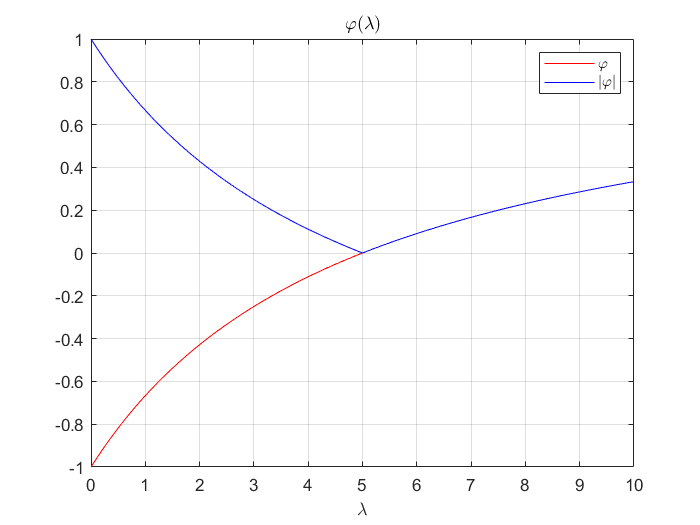
\includegraphics[scale=0.5]{phi_lambda.png}
\caption{Evolution de $\varphi$ et $|\varphi|$ avec $\lambda$}
\label{phi}
\end{figure}

\noindent
D'après Lascaux et Théodore (Tome 2, page 386),
le choix optimal de $\omega$ est celui qui minimise $\Psi(\omega)=\max \{ 
 \frac{\lambda_1-\omega}{\lambda_1+\omega},  \frac{\lambda_M-\omega}{\lambda_M+\omega} \}$
 où $\lambda=1$ et $\lambda_M \approx 4 m^2$.
 
\begin{figure}[h!]
 \centering
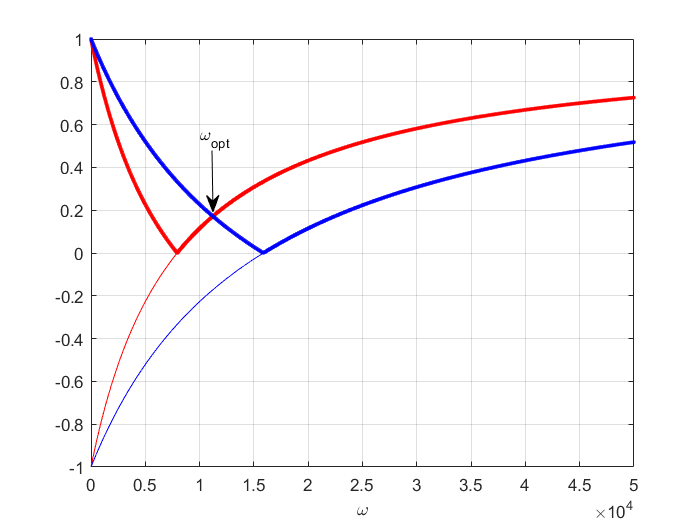
\includegraphics[scale=0.5]{phi_omega.png}
\caption{Evolution de $\varphi$ et $|\varphi|$ avec $\omega$}
\label{phi_omega}
\end{figure}
\noindent
On en déduit que $\omega_{opt}=\sqrt{\lambda_1 \lambda_M} \approx 2m$ (voir Fig. \ref{phi_omega}).

Dans le cas général où $n_x \neq n_y$, on a deux paramètres optimaux qui valent approximativement
$\omega_x=2m_x$ et $\omega_y=2m_y$.

\newpage

\section{Résultats numériques}

\subsection{Convergence}

Le système est discrétisé avec une grille $n_x=64 \times n_y=64$. Le paramètre de
relaxation $\omega$ a été fixé arbitrairement à $256$ et le seuil de tolérance à $\epsilon=10^{-8}$.

La figure \ref{res} représente l'évolution du résidu défini par $||b-Au||_\infty$ en fonction du
nombre d'itérations en échelle semi-logarithmique base 10.
Le résidu décroit de manière exponentielle avec deux régimes différents.
\begin{figure}[h!]
 \centering
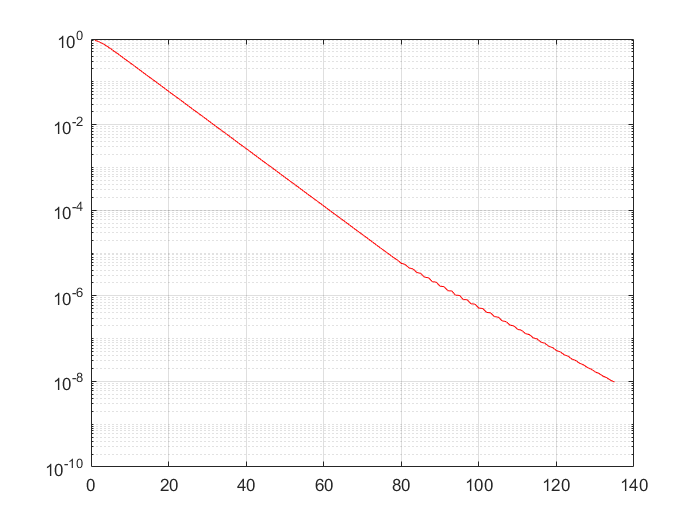
\includegraphics[scale=0.5]{convergence.png}
\caption{Evolution du résidu avec le nombre d'itérations}
\label{res}
\end{figure}

\subsection{Coefficients optimaux}



\subsection{Deux cas tests}

\begin{figure}[h!]
 \centering
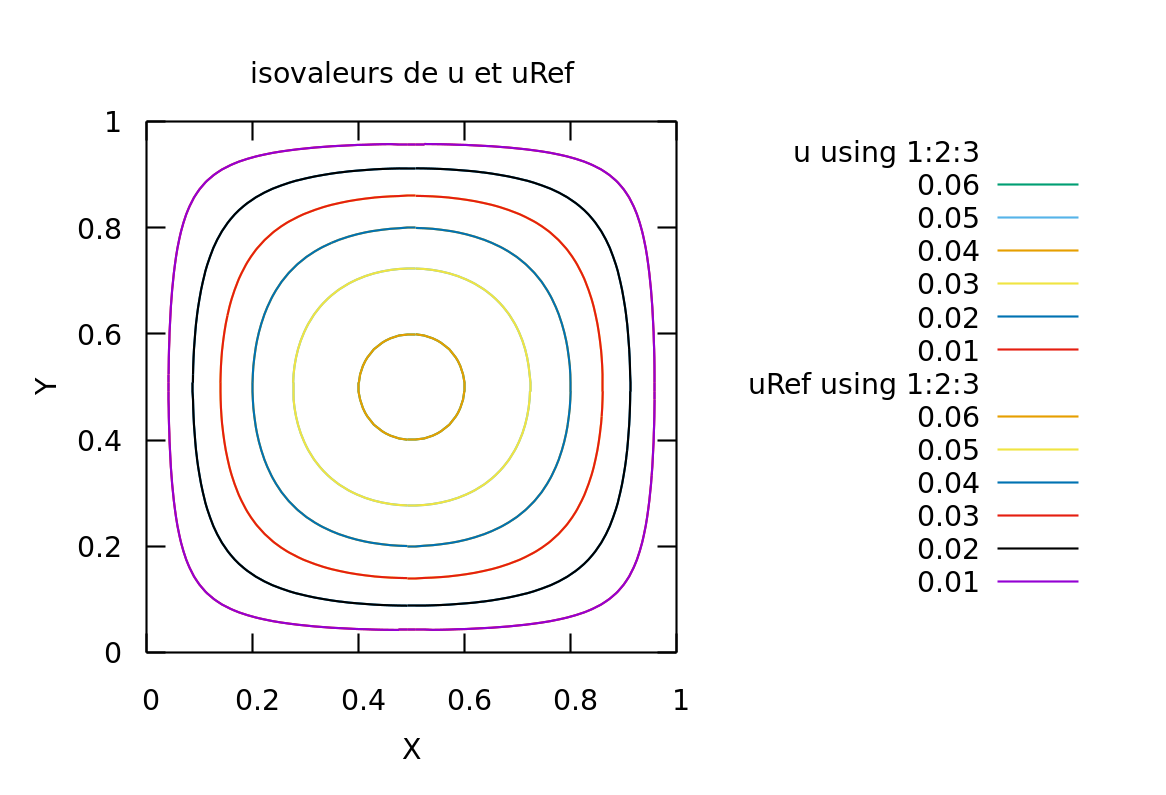
\includegraphics[scale=0.5]{isovaleurs.png}
\caption{Isovaleurs de $u(x,y)$}
\label{iso}
\end{figure}

On n'a traité que des problèmes où la condition de dirichlet aux bords est $u^d=0$.

Le répertoire {\tt Q6/0\_ADI2D} contient le premier cas test où
 $f(x,y) = 2x(1-x) + 2y(1-y)$ s'annulant sur $\partial \Omega$. La solution analytique
vérifiant $\Delta u +f =0$ est $u_{ref}(x,y) = x(1-x) y(1-y)$.
La figure \ref{iso} représente les isovaleurs de la solution numérique $u(x,y)$ et de la solution de référence $u_{ref}(x,y)$. L'accord est excellent.

Le répertoire {\tt Q6/1\_ADI2D} contient le second cas test où
 $f(x,y) = 2 \pi^2 \sin(\pi x) \sin(\pi y)$ qui s'annule sur $\partial \Omega$. La solution analytique
est $u_{ref}(x,y) = \sin(\pi x) \sin(\pi y)$. L'accord est tout aussi parfait.

\gnuscript{iso}{Script gnuplot pour visualiser les isovaleurs}

\subsection{Intérêt de la méthode ADI}

La complexité de la méthode de résolution d'un système tri-diagonale de rang N en utilisant la méthode de décomposition $LU$ est $\vartheta(N)$ et est peu couteuse  par rapport à la méthode
de résolution de Gauss qui a une complexité $\vartheta(N^3)$  pour une matrice dense de rang $N$.

Calculons maintenant la complexité des deux pas fractionnaires de la méthode ADI pour une
grille de taille $n_x \times n_y$.

La première étape revient à résoudre $n_y-2$ petits systèmes linéaires dont la matrice est tri-diagonale de rang $n_x$.
Sa complexité est donc en $\vartheta(n_y \times n_x)$ en ne gardant que l'ordre le plus élevé.

La seconde étape revient à résoudre $n_x-2$ petits systèmes linéaires dont la matrice est tri-diagonale de rang $n_y$.
Sa complexité est donc en $\vartheta(n_x \times n_y)$.

La complexité de la méthode ADI est donc $\vartheta(n_x \times n_y)$.

\subsection{Détermination numérique des paramètres optimaux}

J'ai choisi de prendre $n_x=n_y=64$ et une tolérance $\eps=10^{-6}$.
J'ai repris la fonction polynomiale $f(x,y)$ du premier cas test.

L'évolution du nombre d'itérations en fonction de $\omega \in [64, 464]$ obtenue avec le code
{\tt ADID\_param\_optim} est représenté sur la figure \ref{niter}.

\begin{figure}[h!]
 \centering
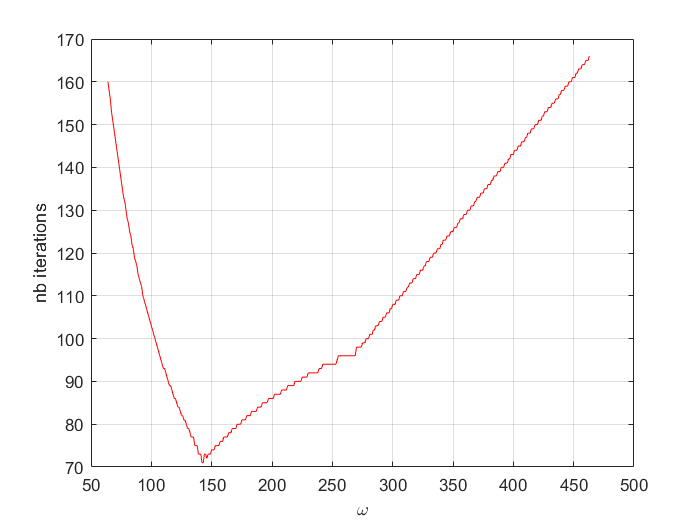
\includegraphics[scale=0.5]{niter_omega.png}
\caption{nombre d'itérations en fonction de $\omega$}
\label{niter}

On obtient une valeur numérique de $\omega_{opt}=142$  supérieure de 10\% à celle estimée théoriquement.

\end{figure}


\end{document}
